\documentclass{article}

\usepackage{amsmath}
\usepackage{graphicx}
\usepackage{bbold}


\title{Examination project 14: Inverse iteration method\\ \small Practical Programming and Numerical Methods 2020}
\author{Marco Majland}
\begin{document}
	\maketitle
	\noindent
	The objective of the project is to iteratively calculate the eigenvalue of a given real symmetric matrix, $A$, closest to an input eigenvalue and its associated eigenvector. This is done using the inverse iteration method which is an improvement of the power iteration method. By shifting the matrix equation of the power method, one obtains the inverse iteration method.\\
	Let $\mathbf{A}$ denote a real  symmetric matrix of dimension $n\times n$ and the initial guess of the eigenvalue and eigenvector be $s$ and $\mathbf{u}$ (normalized), respectively. The inverse iteration method is then given by
	\begin{equation}
		(\mathbf{A} - s\mathbb{1})\mathbf{v} = \mathbf{u}
	\end{equation}
	where $\mathbf{v}$ is the refined eigenvector of $\mathbf{A}$. In the implementation of the inverse iteration algorithm, the above linear matrix equation is solved using QR decomposition.
	\subsection*{Test of convergence relative to deviation from expected eigenvalue}
	The convergence to the expected eigenvalue in the inverse iteration method depends critically on the initial guess. If two eigenvalues of a matrix are very close, of course, there is a high risk for the algorithm to converge to the wrong eigenvalue. This hypothesis is tested in the following way.
	\begin{itemize}
		\item Generate random real symmetrix matrix of size NN
		\item Diagonalize using Jacobi diagonalization procedure
		\item Use initial guess $s_{0} = \delta s_{\textrm{Jacobi}}$ where $s_{0}$ is initial guess of II method, $\delta$ is the deviation and $s_{\textrm{Jacobi}}$ is the Jacobi eigenvalue
		\item Apply II method with $s_{0}$ and corresponding eigenvector as initial guess
		\item Iterate the above procedure for 300 iterations for a given $\delta$
	\end{itemize}
	The above procedure is then repeated for a range of deviations. 
	\begin{figure}
		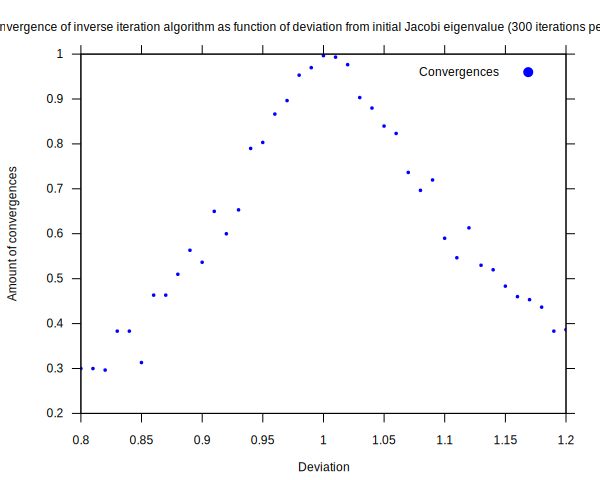
\includegraphics[]{../outfiles/Deviations.pdf}
		\caption{Distributions of convergences. Convergence of 1.0 implies all iterations yielded the expected Jacobi eigenvalue. Convergence of 0.5 implies half of all iterations yielded the expected Jacobi eigenvalue.}
		\label{fig:deviations}
	\end{figure}	
	The resulting normalized distribution is depicted in figure \ref{fig:deviations}. As can be seen, the distribution is symmetric around $\delta = 1.0$ for which the initial guess equals the Jacobi eigenvalues. As expected, the convergence drops rapidly as the deviation differs from 1. For these calculations, the eigenvalue was updated for every iteration using the Rayleigh quotient and updating the QR decomposition.

\begin{thebibliography}{9}
	\bibitem{ref1}
	A. Van Wijngaarden and W. L. Scheen,
	\textit{Table of Fresnel integrals},
	The Computation Department of the Mathematical Centre, Amsterdam,
	1949.
\end{thebibliography}
\end{document}